
% ===============================================
% MATH 34: Multivariable calculus           Spring 2019
% hw_template.tex
% ===============================================

% -------------------------------------------------------------------------
% You can ignore this preamble. Go on
% down to the section that says "START HERE" 
% -------------------------------------------------------------------------

\documentclass{article}

\usepackage[margin=1.5in]{geometry} % Please keep the margins at 1.5 so that there is space for grader comments.
\usepackage{amsmath,amsthm,amssymb,hyperref}
\usepackage{graphicx}
\usepackage{float}
\usepackage{listings}
\usepackage{xparse}
\usepackage{xcolor}
\usepackage{verbatim}

\newcommand{\R}{\mathbf{R}}  
\newcommand{\Z}{\mathbf{Z}}
\newcommand{\N}{\mathbf{N}}
\newcommand{\Q}{\mathbf{Q}}
\newcommand{\C}{\mathbf{C}}
\newcommand{\Log}{\text{Log}}
\newcommand{\Arg}{\text{Arg}}

\newenvironment{theorem}[2][Theorem]{\begin{trivlist}
\item[\hskip \labelsep {\bfseries #1}\hskip \labelsep {\bfseries #2.}]}{\end{trivlist}}
\newenvironment{lemma}[2][Lemma]{\begin{trivlist}
\item[\hskip \labelsep {\bfseries #1}\hskip \labelsep {\bfseries #2.}]}{\end{trivlist}}
\newenvironment{claim}[2][Claim]{\begin{trivlist}
\item[\hskip \labelsep {\bfseries #1}\hskip \labelsep {\bfseries #2.}]}{\end{trivlist}}
\newenvironment{problem}[2][Problem]{\begin{trivlist}
\item[\hskip \labelsep {\bfseries #1}\hskip \labelsep {\bfseries #2.}]}{\end{trivlist}}
\newenvironment{proposition}[2][Proposition]{\begin{trivlist}
\item[\hskip \labelsep {\bfseries #1}\hskip \labelsep {\bfseries #2.}]}{\end{trivlist}}
\newenvironment{corollary}[2][Corollary]{\begin{trivlist}
\item[\hskip \labelsep {\bfseries #1}\hskip \labelsep {\bfseries #2.}]}{\end{trivlist}}

\newenvironment{solution}{\begin{proof}[Solution]}{\end{proof}}

\makeatletter
\newcommand{\skipitems}[1]{%
	\addtocounter{\@enumctr}{#1}%
}
\makeatother

\NewDocumentCommand{\codeword}{v}{%
\texttt{\textcolor{blue}{#1}}%
}


\begin{document}

\large % please keep the text at this size for ease of reading.

% ------------------------------------------ %
%                 START HERE             %
% ------------------------------------------ %

{\Large Page 1 % Replace with appropriate page number 
\hfill  MTH483, Complex Variables, HW3}

\begin{center}
{\Large Wyatt Whiting}
\end{center}
\vspace{0.05in}

% -----------------------------------------------------
% The "enumerate" environment allows for automatic problem numbering.
% To make the number for the next problem, type " \item ". 
% To make sub-problems such as (a), (b), etc., use an "enumerate" within an "enumerate."
% -----------------------------------------------------
\begin{enumerate}
	\item Write the following complex numbers in standard form. Use the principal branch of the logarithm if necessary.
	\begin{enumerate}
		\item $4^i = e^{i\text{Log}{4}}=\cos{\text{Log}(4)}+i\sin{\text{Log}(4)}$
		\item $(1+i\sqrt{3})^{i/2}=e^{i/2\text{Log}(1+i\sqrt{3})}=e^{i/2(\ln|2|+i\arctan{\sqrt{3}})}=e^{-\pi/6 + i(\ln|2|/2)}=e^{-\pi/6}\cos{\frac{\ln|2|}{2}}+ie^{-\pi/6}\sin{\frac{\ln|2|}{2}}$
		\item $(-1)^{\sqrt{2}}=e^{\sqrt{2}(\text{Log}(-1))}=e^{\sqrt{2}(\ln|-1|+i\pi)}=e^{\sqrt{2}\ln 1 + i\pi\sqrt{2}}=\cos{\pi\sqrt{2}}+i\sin{\pi\sqrt{2}}$
		\item $(i-1)^{2i+3}=e^{(2i+3)(\text{Log}(i-1))}=e^{ (2i+3) (\ln\sqrt{2}+i(3\pi/4)) } = e^{ (3\ln\sqrt{2}-(3\pi/2)) +i(2\ln\sqrt{2}+(9\pi/4)) }= e^{3\ln\sqrt{2}-(3\pi/2)} e^{2\ln\sqrt{2}+(9\pi/4)} = 2\sqrt{2}e^{-3\pi/2}e^{i(2\ln\sqrt{2}+(9\pi/4))}$
		
		$=2\sqrt{2}e^{-3\pi/4}\cos{(2\ln\sqrt{2}+(\pi/4))}+i2\sqrt{2}e^{-3\pi/4}\sin{(2\ln\sqrt{2}+(\pi/4))}$
		
		\item $e^{\sin{i}}=e^{i\sinh{1}}=\cos{(\sinh{1})}+i\sin{(\sinh{1})}$
		
		\item $\cos{(-2+i)}=\frac{e^{i(-2+i)}+e^{-i(-2+i)}}{2}=\frac{1}{2} (e^{-1-2i}+e^{1+2i}) $
		
		$=\frac{1}{2}(e^{-1}\cos{(-2)}+ie^{-1}\sin{(-2)}+e\cos{(2)}+ie\sin{(2)})$
		
		$=\frac{1}{2}(e^{-1}\cos{(-2)}+e\cos{(2)})+i\frac{1}{2}(e^{-1}\sin{(2)}+e\sin{(2)})$
		
		\item $\sin{(\pi/4 + i)}=\frac{ e^{i((\pi/4) + i)}-e^{-i((\pi/4) + i)} }{ 2i } = \frac{ e^{(-1 + i(\pi/4))}-e^{(1-i(\pi/4))} }{ 2i }$
		
		$= \frac{ e^{-1}\cos{(\pi/4)}+e^{-1}i\sin{(\pi/4)}-e\cos{(-\pi/4)}-ei\sin{(-\pi/4)} }{ 2i }$
		
		$= \frac{ e^{-1}\cos{(\pi/4)}+e^{-1}i\sin{(\pi/4)}-e\cos{(\pi/4)}+ei\sin{(\pi/4)} }{ 2i }$
		
		$= \frac{ \cos{(\pi/4)}(e^{-1}-e) + i\sin{(\pi/4)}(e^{-1}+e) }{ 2i } $
		
		$= \frac{1}{2}\sin{(\pi/4)}(e^{-1}+e)-\frac{1}{2}i\cos{\pi/4}(e^{-1}-e)$
		
		$= \frac{\cosh{(1)}}{\sqrt{2}}+i\frac{\sinh{(1)}}{\sqrt{(2)}}$
		
		\item $\tan{(\frac{\pi+i}{2})} = \frac{ \sin{((\pi/2) + (i/2))} }{ \cos{((\pi/2) + (i/2))}} = \frac{ \frac{e^{i((\pi/2)+(i/2))} - e^{-i((\pi/2) + (i/2))}}{2i} }{ \frac{e^{i((\pi/2)+(i/2))} + e^{-i((\pi/2) + (i/2))}}{2} }$
		
		$= \frac{e^{(-1/2)+i(\pi/2)}-e^{(1/2)-i(\pi/2)}}{i(e^{(-1/2)+i(\pi/2)}+e^{(1/2)-i(\pi/2)})}$
		
		$= \frac{e^{-1/2}\cos{(\pi/2)}+ie^{-1/2}\sin{(\pi/2)}-e^{1/2}\cos{(-\pi/2)}-ie^{1/2}\sin{(-\pi/2)}}{i(e^{-1/2}\cos{(\pi/2)}+ie^{-1/2}\sin{(\pi/2)}-e^{1/2}\cos{(-\pi/2)}-ie^{1/2}\sin{(-\pi/2)})}$
		
		$= \frac{ie^{-1/2}+ie^{1/2}}{i(ie^{-1/2}-ie^{1/2})}$
		
		$= \frac{e^{-1/2}+e^{1/2}}{ie^{-1/2}-ie^{1/2}}=i\coth{(1/2)}$
		
		\item $\cosh{(1-i(\pi/4))}= \cosh{(1)}\cos{(-\pi/4)}+i\sinh{(1)}\sin{(-\pi/4)}$
		
		$= \frac{\cosh{(1)}}{\sqrt{2}}-i\frac{\sinh{(1)}}{\sqrt{2}}$
		
		\item $\sinh{(1+i\pi)}=\sinh{(1)}\cos{(\pi)}+i\cosh{(1)}\sin{(\pi)} $
		
		$= -\sinh{(1)}+0i$
	\end{enumerate}
	
	\item Find all complex values of the following:
		\begin{enumerate}
			\item $\log{(\sqrt{3}-i})=\ln|2|+i\text{arg}(\sqrt{3}-i)=\ln|2|+i(-\frac{\pi}{6}+2\pi k), k \in \Z$
			
			\item $\log{(-ie)}=\ln|e|+i\text{arg}(-ie)=1+i(-\frac{\pi}{2}+2\pi k), k \in \Z$
			
			\item $\arcsin{(1+i)} = \frac{1}{i}\ln(i(1+i)+|1-(1+i)^2|^{1/2}e^{(i/2)(\text{arg}(1-(1+i)^2)})$
			
			$=\frac{1}{i}\ln((-1+i)+\sqrt{5}^{1/2}e^{(i/2)\text{arg}(1-2i)})$
			
			$=\frac{1}{i}\ln((-1+i)+\sqrt{5}^{1/2}e^{(i/2)(\arctan{(2)}+2\pi k)})$
			
			$=\frac{1}{i}\ln((-1+i)+5^{1/4}e^{i(\frac{\arctan{(2)}+2\pi k}{2})})$
			
			$=-i\ln((-1+i)+\sqrt{1-2i})$
		\end{enumerate}
		
	\item Determine if each of the following statements is true. If it is, prove it. If it is not, give a counterexample.
		\begin{enumerate}
			\item \textit{Counterexample}: Let $z=-\frac{1}{\sqrt{5}}-i\frac{2}{\sqrt{5}}$. Then we have:
			
			\[  \sqrt{-\frac{1}{\sqrt{5}}-i\frac{2}{\sqrt{5}}} =e^{\frac{1}{2}(\ln|1|+i(\arctan(2)-\pi))}  \]
			
			\[  =e^{\frac{1}{2}(i\arctan(2)-i\pi)}   \]
			
			\[  =e^{-i\frac{\pi}{2}}e^{\frac{1}{2}(i\arctan(2))}   \]
			
			\[  =-ie^{\frac{1}{2}(i\arctan(2))}   \]
			
			\[  =-i\sqrt{\frac{1}{\sqrt{5}}+i\frac{2}{\sqrt{5}}}=-i\sqrt{-z} \neq i\sqrt{z}   \]
			

			
			
			\item \textit{Proof}: Let $z \in \C$ be arbitrary. Then $\sin^2(z)+cos^2(z)=(\frac{e^{iz}-e^{-iz}}{2i})^2 + (\frac{e^{iz}+e^{-iz}}{2})^2=\frac{e^{2iz}-2+e^{-2iz}}{-4}+\frac{e^{2iz}+2+e^{-2iz}}{4}=\frac{4}{4}=1$. This proves $\sin^2(z)+\cos^2(z)=1$.
			
			\item \textit{Counterexample}: Let $z=i$. Then we have $|\cos(i)|^2+|\sin(i)|^2=| \frac{e^{-1}+e^{1}} {2} |^2+| \frac{e^{-1}-e^{1}} {2i} |^2=$. It's is clear that $|\frac{e^-1+e}{2}|^2=\frac{e^{-2}+2+e^2}{4}\geq 1$, so the sum is already greater than 1. Thus $|\cos(i)|^2+|\sin(i)|^2 \neq 1$.
			
			\item \textit{Proof}: Let $z = a+bi \in \C$ be arbitrary. Then we have $\sin(a+bi+2\pi)=\sin(a+2\pi)\cosh(b)+i\cos(a+2\pi)\sinh(b)=\sin(a)\cosh(b)+i\cos(a)\sinh(b)=\sin(a+bi)=sin(z)$. This proves $\sin(z+2\pi)=\sin(z)$.
			
			\item \textit{Proof}: Let $z = a+bi \in \C$ be arbitrary. Then we have $\sin(\pi-a-bi)=\sin(\pi-a)\cosh(-b)+i\cos(\pi-a)\sinh(-b)=\sin(a)\cosh(-b)+i\cos(a)\sinh(-b)=\sin(a)\cosh(b)+i\cos(a)\sinh(b)=\sin(a+bi)=sin(z)$. This proves $\sin(\pi-z)=\sin(z)$.
			
			\item \textit{Proof}: Let $z = a+bi \in \C$ be arbitrary. Then $e^{\overline{z}}=e^{\overline{a+bi}}=e^{a-bi}=e^a\cos(-b)+e^ai\sin(-b)=e^a\cos(b)-e^ai\sin(b)=\overline{e^a\cos(b)+e^ai\sin(b)}=\overline{e^{a+bi}}=\overline{e^z}$. This proves $e^{\overline{z}}=\overline{e^z} $
		\end{enumerate}
		
	\item $f(z)=z^{1/4}, f(1)=1^{1/4}=-i$
	
	$f(1)=e^{\frac{1}{4}(\ln|1|+i\text{arg}(1))}=e^{\frac{1}{4}(i(0+2\pi k))}=e^{i\frac{k\pi}{2}0}=-i $
	
	$e^{i\frac{k\pi}{2}0}=-i=e^{i\frac{-\pi}{2}} \implies k=-1$
	
	So we have $f(x)=e^{i\frac{-\pi}{2}}z^{1/4}$ where $z^{1/4}$ takes the principle value.
	
	So thus $f(x)=e^{i\frac{-\pi}{2}}(4i)^{1/4}=e^{i\frac{-\pi}{2}}e^{\frac{1}{4}(\ln|4i|+i\text{Arg}(4i))}=e^{i\frac{-\pi}{2}}e^{\frac{\ln2}{2}+i\frac{\pi}{8}}=e^{-i\frac{3\pi}{8}+\frac{\ln2}{2}}$
	
	$=\sqrt{2}(\cos(-3\pi/8)+i\sin(-3\pi/8))$,
	
	\item $f(z)=\sqrt{z-1}\sqrt[3]{z-i}$. Since the domain of the root functions depend on the domain of Log($z$), then we have that $z-1\leq0$ and $z-i\leq 0$ must be excluded from the domain of f($z$). Thus $z \leq 1$ and $z \leq i$ must be excluded. Although $\C$ is not an ordered field, we take this notation to mean that the rays pointing in the negative real direction from both 1 and i must be excluded from the domain of f($z$).
	
	\item
	\begin{enumerate}
		\item log($z^5$)
		
		We will use the principle argument when defining this logarithm. So we cut the plane along $\{ z : \text{Arg}(z)=-\pi \}\cup\{0\}$, defining the domain of the logarithm. So then $z^5$ cannot a negative real number or 0. The argument of such a number is $-\pi$, so the argument of $z$ cannot be $-\frac{\pi}{5}$. So we must omit from the domain of log($z^5$) the ray emanating from the origin with principle argument $-\frac{\pi}{5}$ including the origin itself, giving us the function f($z$)=Log($z^5$).
		
		\[ f(1+2i)=\Log(1+2i)=\ln|25\sqrt{5}|+i\Arg(41-38i) \]
		
		\[ =\ln|25\sqrt{5}|+i\arctan(-\frac{38}{41})\]
		
		\[ f(-2+i)=\Log(-2+i)=\ln|25\sqrt{5}|+i\Arg(38+41i) \]
		
		\[ =\ln|25\sqrt{5}|+i\arctan(\frac{38}{41})\]
		
		\[ \text{So } f(1+2i)=\overline{f(-2+i)}\]
		
		\item log($z^2+1$)
		
		We will use the same cutting method as above for $\Log$, so we have that $z^2+1$ cannot be a negative real number or 0. This is to say that $\Arg(z^2+1)=\Arg((z+i)(z-i))=\Arg(z+i)+\Arg(z-i)(\text{mod } 2\pi)\neq -\pi$. We may then choose the argument of our cuts from coming from $i$ and $-i$ to be arbitrary as long as their sum of their principle arguments mod $2\pi$ to be -pi. Thus our cuts will be along the ray extending from $i$ with principle argument 0 and along the ray extending from $-i$ with argument $-\pi$.
		
		\[f(1+2i)=\Log(1+2i)=\ln|2\sqrt{5}|+i\Arg(-2-4i)  \]
		
		\[ =\ln|2\sqrt{5}+i(\text{Arctan}(2)-\pi) \]
		
		\[f(-2+i)=\Log(-2+i)=\ln|2\sqrt{5}|+i\Arg(4-4i)  \]
		
		\[ =\ln|2\sqrt{5}+i(\text{Arctan}(-1)) \]
	\end{enumerate}
	
	\item 
		\begin{enumerate}
			\item \codeword{ParametricPlot[{Re[Sin[x + I y]], Im[Sin[x + I y]]}, {x, -Pi/2, Pi/2}, {y, -1, 1}]}
			
			\begin{figure}[H]
			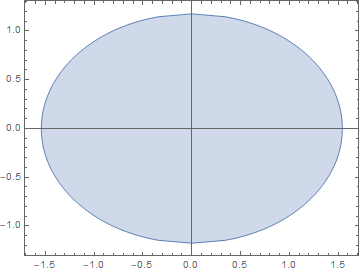
\includegraphics[scale=0.8]{image1.png}
			\end{figure}
			
			\item \codeword{ParametricPlot[{Re[Sin[x + I y]], Im[Sin[x + I y]]}, {x, -Pi]/2, Pi]/2}, {y, -1, 1}, PlotRange -> Full, Mesh -> Automatic, MeshStyle -> {Red, Green}]}
			
			\begin{figure}[H]
			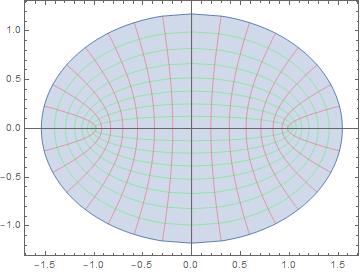
\includegraphics[scale=0.8]{image2.png}
			\end{figure}
			
			Based on this picture, it appear that the function maps the lines $x=\frac{\pi}{2}$ to $\{ z \in \C: z = a + 0i, a \geq 1\}$ and $x=-\frac{\pi}{2}$ to $\{ z \in \C: z = a + 0i, a \leq -1\}$.
			
			\item Let's examine side-by-side figures of the rectangle and its image.
			\begin{figure}[H]
			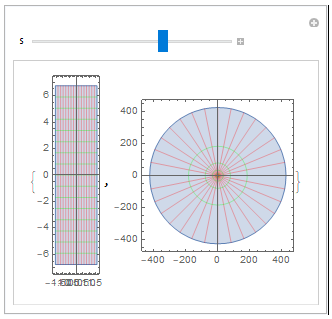
\includegraphics[scale=1.0]{image3.png}
			\end{figure}
			
			We can see that having a taller rectangle causes the image to become wider and wider without overlaps because the background blue remains the same color. Therefore the rectangle $[-\frac{\pi}{2}, \frac{\pi}{2}]\times[-\infty,\infty]$ maps onto the entire complex plane. This is not one-to-one as the line $x=\frac{\pi}{2}$ must fold onto itself. i.e. $\sin((\pi/2) + i)=\sin((\pi/2) - i)$. 
			
			\item If we now consider the open vertical strip $(-\frac{\pi}{2}, \frac{\pi}{2})\times[-\infty,\infty]$, then the problematic lines $x=\frac{\pi}{2}$ and $x=-\frac{\pi}{2}$ are no longer an issue, so this will map onto $\C\setminus\{ z\in\C: z = a + 0i, |a|\geq1\}$. With those rays removed, the mapping is now one-to-one over the open rectangle.
		\end{enumerate}
\end{enumerate}

% ---------------------------------------------------
% Anything after the \end{document} will be ignored by the typesetting.
% ----------------------------------------------------

\end{document}

